\documentclass[11pt]{article}

\usepackage[margin=1in]{geometry}
\usepackage{amsmath,amssymb,mathtools}
\usepackage{booktabs}
\usepackage{enumitem}
\usepackage{graphicx}
\usepackage{hyperref}
\usepackage{xcolor}
\usepackage{listings}

\hypersetup{
  colorlinks=true,
  linkcolor=blue,
  citecolor=blue,
  urlcolor=blue
}

\lstset{
  basicstyle=\ttfamily\small,
  breaklines=true,
  columns=fullflexible,
  frame=single,
  xleftmargin=0.5em,
  xrightmargin=0.5em
}

\graphicspath{{docs/}{./}}

\title{Sequence-Edit JEPA and Masked Denoising Baselines:\\Chronology, Methods, Results, and Next Experiments}
\author{Internal Research Note}
\date{May 17, 2026}

\begin{document}
\maketitle

\begin{abstract}
This note records the current state of the sequence-editing experiments in this
repository.  The project began with a fixed-length action-conditioned JEPA model
for symbolic denoising and editing, then added denoising language-model and
causal language-model baselines on LANO and iGSM.  The first iGSM full-denoise
results showed that the causal LM was much stronger than both denoising models;
JEPA weakly beat the original denoising LM, but the denoising LM often left mask
tokens in the output.  A literature review of D3PM, MDLM/MD4, SEDD, SMDM, and
LLaDA identified several mismatches: the denoising target was often $x_{t-1}$
rather than $x_0$, the loss included visible tokens, the policy was asked to
guess a hidden reveal order, and the sampler allowed \texttt{[MASK]} as a clean
prediction.  We implemented an $x_0$ masked-diffusion objective, mask-logit
suppression, corrected JEPA full-denoise inference through its latent predictor,
fixed-$k$ commit ablations, and new stepwise JEPA corruption modes.  This
document gives the precise math and the experimental chronology so a reader can
reconstruct what was done and why.
\end{abstract}

\section{Chronology}

\paragraph{Initial controlled task: LANO.}
LANO was used as the first reconstruction/editing diagnostic because it has a
small grammar and unambiguous exact-reconstruction metrics.  At 200k mask
training steps, Sequence-Edit JEPA and the denoising LM both reached about
63\% exact reconstruction, about 95\% token accuracy, and about 56\% grammar
validity.  This established that the basic bidirectional denoising machinery was
working on a controlled task.

\paragraph{iGSM baselines.}
We then trained three iGSM medium-difficulty baselines to checkpoint 200k:
causal LM generation, denoising LM full denoise, and action-conditioned JEPA
full denoise.  Job \texttt{3605092\_[0-2]} completed the final training
resumes.  Job \texttt{3605200} produced the first trusted latest-checkpoint
full-denoise evaluation.

\paragraph{The first iGSM read.}
The causal LM was clearly strongest.  JEPA beat the original denoising LM under
full denoise, but only weakly, and it remained far below causal generation.  The
plain denoising LM initially scored zero answer accuracy because it frequently
kept or committed \texttt{[MASK]} tokens.

\paragraph{LANO replacement.}
Job \texttt{3605204} trained LANO replacement correction.  It had high edit
precision but very low edit recall, so the model was conservative: when it
edited, it was usually right, but it missed most required edits and had poor
grammar validity.  This made replacement correction a debugging task rather than
something ready for iGSM.

\paragraph{Literature-driven denoising fix.}
A review of modern discrete diffusion LMs identified the main mismatch.  SOTA
masked diffusion models are clean-token predictors: given a partially masked
sequence $x_t$, predict $x_0$ on corrupted positions only.  The reverse sampler
chooses how many positions to reveal; the token head is not trained to output
\texttt{[MASK]}.  We therefore changed mask/replacement corruptors to support
$x_t \rightarrow x_0$ training, restricted token CE to corrupted editable
positions, suppressed \texttt{[MASK]} as an editable prediction, and increased
the noising step count for iGSM x0 configs.

\paragraph{JEPA inference correction.}
The next important discovery was that the full-denoise evaluator did not use
JEPA as a latent predictive model.  It encoded $x_t$, ran the policy, and took
tokens directly from the policy token head.  The latent predictor and decoder
were bypassed.  On May 15, 2026, full-denoise JEPA inference was changed so the
default path is:
\[
  h_t = f_\theta(x_t,t), \quad
  \hat{a}_t = \pi_\theta(h_t), \quad
  \hat{h}_{t'} = g_\theta(h_t,\hat{a}_t,t), \quad
  p_\theta(x_{t'} \mid x_t) = d_\theta(\hat{h}_{t'}).
\]
The old policy-head token path remains available only as an ablation.

\paragraph{Current submitted jobs.}
The x0 iGSM resume and eval arrays completed.  The x0 denoising LM is now the
strongest denoising-style iGSM baseline, while x0 JEPA remains below it.  The
first stepwise allocation timed out cleanly after checkpoint 120k for all four
variants, and the dependent resume completed to checkpoint 200k for T20/T50/T64
mask and T64 replacement.  Follow-up diagnostic status as of May 19, 2026 is:
\begin{itemize}[leftmargin=*]
\item \texttt{3615623\_[0-2]}: proposal coverage, factorized oracle, and
  DLM-token proposer diagnostics completed.
\item \texttt{3615624\_[0-15]}: larger oracle-MPC grid over horizon,
  candidate count, token count, and latent vs re-encode rollout completed.
\item \texttt{3615625\_[0-1]}: lightweight value-head training to regress
  oracle-goal latent energy completed.
\item \texttt{3615643\_[0-1]}: rollout-repair continuation from latest T20/T50
  checkpoints with a 20k-step diagnostic budget completed.  Earlier repair submissions
  \texttt{3615626} and \texttt{3615630} were replaced after fixing the Hydra
  override and reducing the budget.
\item \texttt{3621296\_[0-7]}: objective/capacity ablations are live.  All
  eight tasks are running after the array throttle was raised from
  \texttt{\%2} to \texttt{\%8}.  Resume array
  \texttt{3624400\_[0-7]} is queued because the slower variants will not reach
  200k in one allocation, and the dependent MPC eval now waits for that resume.
\end{itemize}

\section{Notation and Tasks}

Let $x_0 = (x_0^1,\ldots,x_0^L)$ be a clean token sequence, $m \in \{0,1\}^L$
an editable mask, and $p \in \{0,1\}^L$ an attention mask.  For iGSM, prompt
tokens are visible and non-editable; solution and answer tokens are editable.
For LANO, the editable region is the expression to reconstruct or repair.  We
write $E=\{i:m_i=1,p_i=1\}$ for editable non-padding positions.

The main iGSM metric is answer accuracy, computed by extracting the predicted
\texttt{<igsm\_answer>} span and comparing it with the gold answer token ids.
We also track exact sequence match, token accuracy, and qualitative
multi-step denoising traces.

\section{Forward Corruption}

\subsection{Masked x0 Corruption}

The modern masked-diffusion version samples a corrupted set $C_t \subseteq E$.
This repo currently uses exact uniform corruption counts:
\[
  c \sim \mathrm{Uniform}\{1,\ldots,|E|\}, \qquad |C_t|=c,
\]
with positions sampled uniformly without replacement.  A continuous or integer
timestep is assigned by inverting a cumulative mask schedule:
\[
  t = \gamma^{-1}\left(\frac{|C_t|}{|E|}\right),
\]
where the cosine schedule is
\[
  \gamma(t) = \sin^2\left(\frac{\pi t}{2T}\right).
\]
The masked input is
\[
  x_t^i =
  \begin{cases}
    \texttt{[MASK]} & i \in C_t,\\
    x_0^i & \text{otherwise.}
  \end{cases}
\]
The clean x0 target is $x_0$, but token CE is only charged on $C_t$.

\subsection{Replacement x0 Corruption}

Replacement uses the same corrupted set $C_t$, but replaces positions with
random non-special vocabulary tokens:
\[
  x_t^i =
  \begin{cases}
    r^i, \quad r^i \neq x_0^i & i \in C_t,\\
    x_0^i & \text{otherwise.}
  \end{cases}
\]
This tests visible-token correction rather than unmasking.  The x0 replacement
LANO run improved edit recall but still had weak exact reconstruction and
grammar, so replacement remains diagnostic.

\subsection{Stepwise Corruption}

For stepwise JEPA, we intentionally do not target $x_0$ in one jump.  Given a
current corrupted set $C_t$, the corruptor chooses a deterministic visible
reveal set $R_t \subseteq C_t$.  In the current implementation, $R_t$ is the
left-to-right prefix of currently corrupted positions with size
\[
  |R_t| = \min\left(|C_t|,\left\lceil \frac{|E|}{T}\right\rceil\right).
\]
The next state is
\[
  x_{t'}^i =
  \begin{cases}
    x_0^i & i \in R_t,\\
    x_t^i & \text{otherwise,}
  \end{cases}
  \qquad
  t'=\gamma^{-1}\left(\frac{|C_t|-|R_t|}{|E|}\right).
\]
This avoids the old hidden-random-reveal-order target.  The reveal set is
identifiable from $x_t$ and position, so the policy can learn a concrete edit
order.  Positions in $R_t$ are labeled \textsc{Replace}; other editable
positions are labeled \textsc{Keep}.

\section{Models and Losses}

\subsection{Denoising LM}

The denoising LM is a bidirectional Transformer encoder with token, segment, and
timestep embeddings, followed by a token decoder:
\[
  h_t = f_\theta(x_t,t), \qquad
  \ell_\theta^i = d_\theta(h_t^i).
\]
The x0 masked-diffusion loss is
\[
  \mathcal{L}_{\mathrm{DLM}}
  =
  \mathbb{E}_{x_0,C_t}
  \left[
    -\frac{1}{\max(1,|C_t|)}
    \sum_{i \in C_t}
    \log p_\theta(x_0^i \mid x_t,t)
  \right].
\]
The \texttt{[MASK]} logit is suppressed for editable clean-token predictions.
The key difference from the original baseline is that visible tokens no longer
dominate the loss, and masked positions are never trained to remain masked.

\subsection{Sequence-Edit JEPA}

Sequence-Edit JEPA has four main components:
\begin{itemize}[leftmargin=*]
\item online encoder $f_\theta$ for the current state;
\item EMA target encoder $\bar f$ for the target state;
\item action policy $\pi_\theta$, producing op logits and action-token logits;
\item latent predictor $g_\theta$ and token decoder $d_\theta$.
\end{itemize}

The action-conditioned latent predictor receives the current latent state and
an action embedding.  In the current code, the action embedding is the sum (or
concat-projected form, depending on config) of a timestep embedding, an op
embedding, and a token embedding:
\[
  e(a_i,t) =
  e_{\mathrm{time}}(t) +
  e_{\mathrm{op}}(a_i^{\mathrm{op}}) +
  e_{\mathrm{tok}}(a_i^{\mathrm{tok}}).
\]
For x0 mask JEPA, corrupted positions are labeled
\[
  a_i = (\textsc{Replace}, x_0^i), \quad i \in C_t,
\]
and uncorrupted editable positions are \textsc{Keep}.  For stepwise JEPA,
only $i\in R_t$ are \textsc{Replace}; unrevealed positions in $C_t\setminus R_t$
are \textsc{Keep}.

The latent prediction is
\[
  h_t = f_\theta(x_t,t), \qquad
  \hat h_{t'} = g_\theta(h_t,a_t,t).
\]
The target latent is encoded by the EMA encoder:
\[
  \bar h_{t'} = \bar f(x_{t'},t').
\]
The JEPA dynamics loss is a masked mean-squared error after projection:
\[
  \mathcal{L}_{\mathrm{dyn}} =
  \frac{1}{\sum_i p_i}
  \sum_{i:p_i=1}
  \left\|
    P_\theta(\hat h_{t'}^i) - \bar P(\bar h_{t'}^i)
  \right\|_2^2.
\]
The decoder token loss is
\[
  \mathcal{L}_{\mathrm{tok}} =
  -\frac{1}{|M_{\mathrm{tok}}|}
  \sum_{i\in M_{\mathrm{tok}}}
  \log p_\theta(x_{t'}^i \mid \hat h_{t'}^i),
\]
where $M_{\mathrm{tok}}=C_t$ for x0 mask JEPA and $M_{\mathrm{tok}}=R_t$ for
stepwise JEPA.  The action loss is the sum of op CE and token CE for action
tokens on editable positions.  The total loss is
\[
  \mathcal{L}_{\mathrm{JEPA}}
  =
  \lambda_{\mathrm{act}}\mathcal{L}_{\mathrm{act}}
  +
  \lambda_{\mathrm{dyn}}\mathcal{L}_{\mathrm{dyn}}
  +
  \lambda_{\mathrm{tok}}\mathcal{L}_{\mathrm{tok}}
  +
  \lambda_{\mathrm{sig}}\mathcal{L}_{\mathrm{sigreg}}.
\]

\subsection{Exact Difference: Denoising LM vs JEPA}

The denoising LM directly predicts clean tokens from encoded $x_t$:
\[
  x_t \xrightarrow{f_\theta} h_t \xrightarrow{d_\theta} \hat x_0.
\]
JEPA predicts an action-conditioned next latent state, then decodes:
\[
  x_t \xrightarrow{f_\theta} h_t,\quad
  h_t \xrightarrow{\pi_\theta} \hat a_t,\quad
  (h_t,\hat a_t) \xrightarrow{g_\theta} \hat h_{t'},\quad
  \hat h_{t'} \xrightarrow{d_\theta} \hat x_{t'}.
\]
Thus JEPA is not merely denoising plus an extra MSE term when evaluated
correctly.  Its deployed token prediction should come from the predicted latent
state, not directly from the policy token head.  The old evaluator violated
this, which is why \texttt{policy\_head} is now only an ablation.

\section{Sampling}

\subsection{Scheduled Commit Sampler}

Full denoise starts from all editable positions masked.  At step $t$, the model
predicts token logits and a confidence score for every remaining mask.  The
scheduled sampler computes the target number of remaining masks under
$\gamma(t-1)$ and commits the highest-confidence positions needed to reach that
count.  At the final step, all remaining positions are force-filled with
non-mask predictions.

\subsection{Fixed-$k$ Sampler}

The fixed-$k$ sampler commits exactly $k$ positions per sequence per reverse
iteration, except at the end.  It uses the current remaining mask ratio to
choose a timestep:
\[
  t = \gamma^{-1}\left(\frac{\#\text{remaining masks}}{|E|}\right).
\]
Submitted eval jobs compare \texttt{commit\_k=1,2,5,10} to the scheduled
sampler.  The hypothesis is that $k=1$ may avoid simultaneously committing
incompatible tokens, while larger $k$ is faster but may propagate early errors.

\section{Results}

\subsection{LANO Mask at 200k}

\begin{table}[h]
\centering
\begin{tabular}{lrrrr}
\toprule
Model & Exact & Token Acc. & Grammar & Parse Depth \\
\midrule
Sequence-Edit JEPA & 62.79 & 94.65 & 56.30 & 81.30 \\
Denoising LM & 62.74 & 95.50 & 55.86 & 83.78 \\
Causal LM generation & 0.00 & 19.97 & 45.12 & -- \\
\bottomrule
\end{tabular}
\caption{LANO mask reconstruction.  The causal setup is generation, not the same
conditional reconstruction problem.}
\end{table}

\subsection{iGSM Full-Denoise, Job 3605200}

\begin{table}[h]
\centering
\begin{tabular}{lrrrrrr}
\toprule
Model & ID & OOD ops & op20 & op21 & op22 & op23 \\
\midrule
Causal LM & 88.3 & 86.7 & 25.8 & 27.3 & 15.6 & 15.6 \\
JEPA full denoise & 29.7 & 28.1 & 6.3 & 12.5 & 7.0 & 6.3 \\
Denoising LM full denoise & 0.0 & 0.0 & 0.0 & 0.0 & 0.0 & 0.0 \\
\bottomrule
\end{tabular}
\caption{Answer accuracy percentages from
\texttt{latest\_full\_denoise\_metrics\_3605200.summary.json}.}
\end{table}

\subsection{iGSM Rerun with Corrected Sampler Path}

Jobs \texttt{3605202} and \texttt{3605203} later completed.  Causal and JEPA
values matched the 3605200 snapshot, while the denoising LM became nonzero:
\begin{table}[h]
\centering
\begin{tabular}{lrrrrrr}
\toprule
Model & ID & OOD ops & op20 & op21 & op22 & op23 \\
\midrule
Denoising LM, corrected sampler path & 22.7 & 21.9 & 5.5 & 5.5 & 4.7 & 4.7 \\
\bottomrule
\end{tabular}
\caption{The old denoising LM remains weak, but suppressing committed
\texttt{[MASK]} tokens materially changes the answer metric.}
\end{table}

\subsection{iGSM x0 Full-Denoise, Job 3607176}

The x0 objective changes the denoising conclusion.  The denoising LM is now the
strongest denoising-style baseline, and JEPA predictor-decoder inference does
not yet beat it.
\begin{table}[h]
\centering
\begin{tabular}{lrrrrrr}
\toprule
Model & ID & OOD ops & op20 & op21 & op22 & op23 \\
\midrule
Causal LM & 88.3 & 86.7 & 25.8 & 27.3 & 15.6 & 15.6 \\
x0 JEPA predictor-decoder & 32.8 & 28.9 & 3.9 & 5.5 & 3.9 & 7.8 \\
x0 Denoising LM & 42.2 & 29.7 & 9.4 & 8.6 & 6.2 & 9.4 \\
\bottomrule
\end{tabular}
\caption{Answer accuracy percentages from
\texttt{x0\_latest\_full\_denoise\_metrics\_3607176.summary.json}.}
\end{table}

The x0 commit ablation \texttt{3612686} showed that JEPA \texttt{policy\_head}
can improve ID accuracy but hurts long-op OOD.  The predictor-decoder path is
still the better JEPA OOD setting.  For the denoising LM, \texttt{commit\_k=1}
is worth a larger rerun because several fixed long-op splits improved.

\subsection{Stepwise JEPA Diagnostics}

Stepwise JEPA trains on next-state denoising rather than direct x0 prediction.
By 120k, T20/T50 have strong one-step edit F1 but weak generation.  The partial
commit sweep \texttt{3614356} is diagnostic rather than final because different
array elements saw different latest checkpoints, but its message is stable:
small-k commits and the smaller policy head help slightly and do not solve
long fixed-op generation.
\begin{table}[h]
\centering
\begin{tabular}{lrrl}
\toprule
Run/mode & ID & OOD ops & Fixed-op note \\
\midrule
T20 policy head, $k=1$ & 9.4 & 10.9 & op20 1.6; op21--23 0.0 \\
T20 policy head, schedule & 6.2 & 10.9 & op20--23 all 0.0 \\
T20 predictor-decoder, $k=1$ & 6.2 & 6.2 & op20--23 all 0.0 \\
T50 predictor-decoder, $k=5$ & 1.6 & 3.1 & op20 4.7; op21 3.1; op23 1.6 \\
\bottomrule
\end{tabular}
\caption{Selected answer accuracies from the partial stepwise commit sweep.}
\end{table}

Oracle-goal latent MPC \texttt{3614357} is the more informative diagnostic.
Without oracle-token candidate injection, answer accuracy remains near zero.
With the correct token forced into the candidate set, the latent-energy scorer
solves small ID/OOD diagnostics: T20 reaches 100\% ID and 75\% aggregate OOD on
the small batches.  Fixed op20/op23 entries were capped by \texttt{max\_steps}
and left many masks, so they are not a clean comparison.  The conclusion is that
proposal/token coverage is now a prime bottleneck.

Proposal/factorized diagnostics \texttt{3615623} completed on May 18, 2026.
For T50, the oracle action is usually present in the candidate set:
top-16 position recall is 100\% on ID/OOD ops and remains above 98\% on
op20/op23, while top-20 token recall is about 93--98\%.  The factorized oracle
is more decisive: model positions plus oracle tokens reach 93.8\% ID and
67--72\% OOD ops, while oracle positions plus model tokens remain near the
model/model baseline.  The deployable bottleneck is therefore token choice and
scoring, not only position selection.

DLM-token proposal improves the deployable sampler but does not close the gap:
model positions plus x0-DLM tokens reach 39.1\%/26.6\% ID/OOD ops for T20 and
37.5\%/29.7\% for T50.

The 20k rollout-repair diagnostic \texttt{3615643} completed.  T20 improved to
17.2\% ID full-denoise answer accuracy, with op20/op23 still only
0.8\%/2.3\%.  T50 remained weak at 3.1\% ID and 0\% on the fixed long-op
splits.

\subsection{Curves and Artifacts}

\begin{figure}[h]
\centering
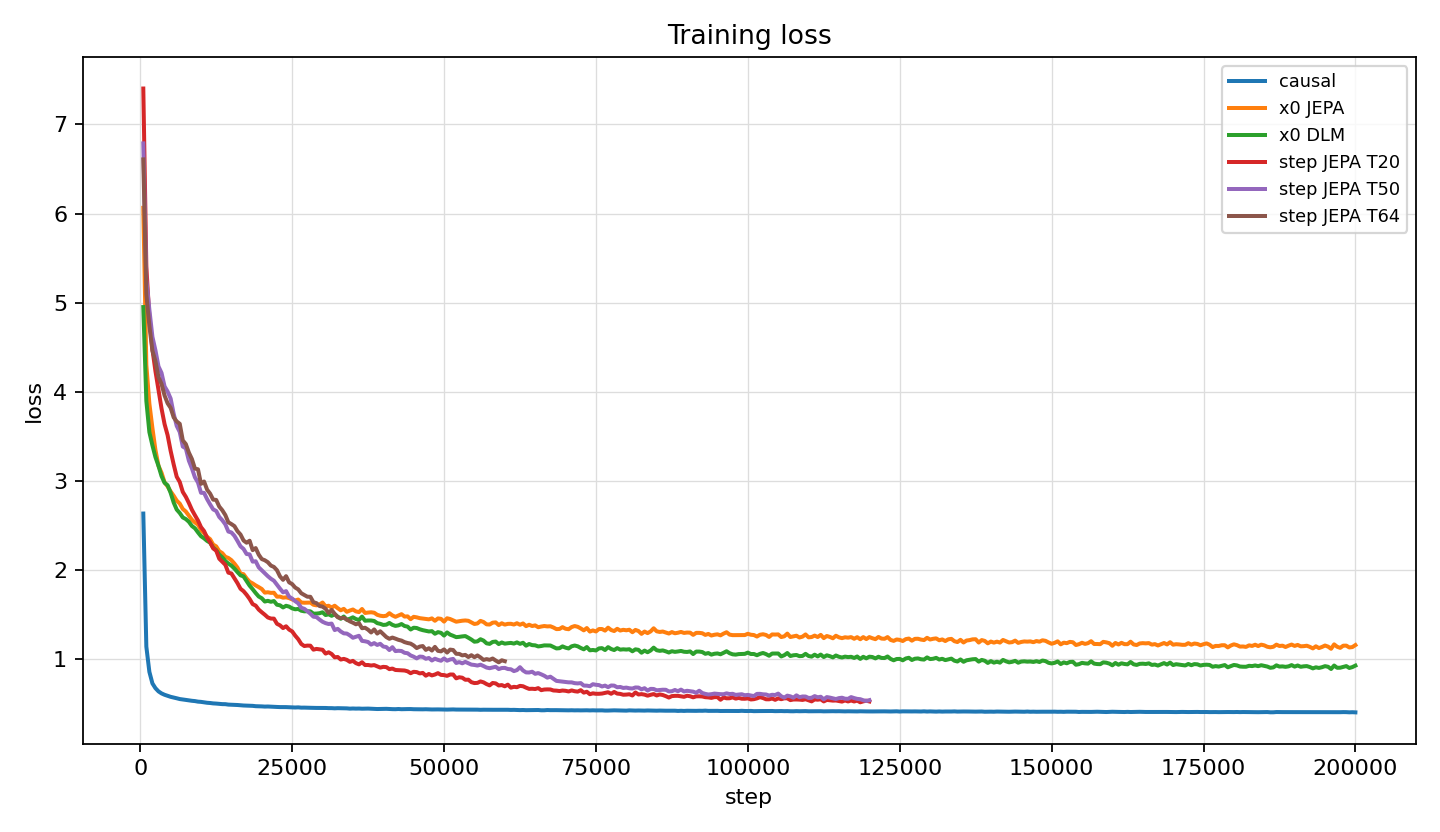
\includegraphics[width=\linewidth]{assets/igsm_train_loss.png}
\caption{Training loss curves extracted from latest checkpoint trainer states.}
\end{figure}

\begin{figure}[h]
\centering
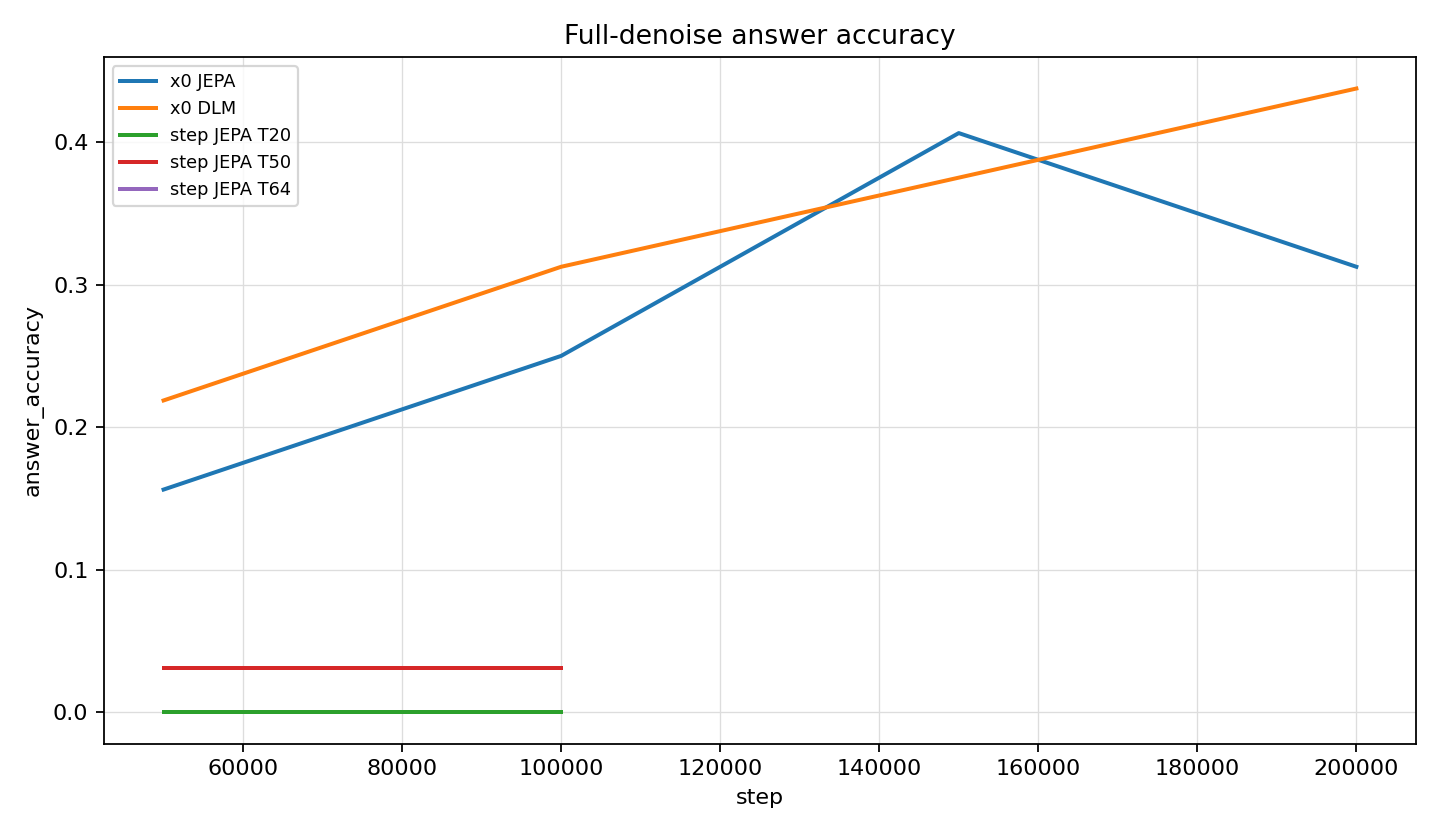
\includegraphics[width=\linewidth]{assets/igsm_full_denoise_answer_accuracy.png}
\caption{Periodic full-denoise answer accuracy for the major iGSM runs.}
\end{figure}

\begin{figure}[h]
\centering
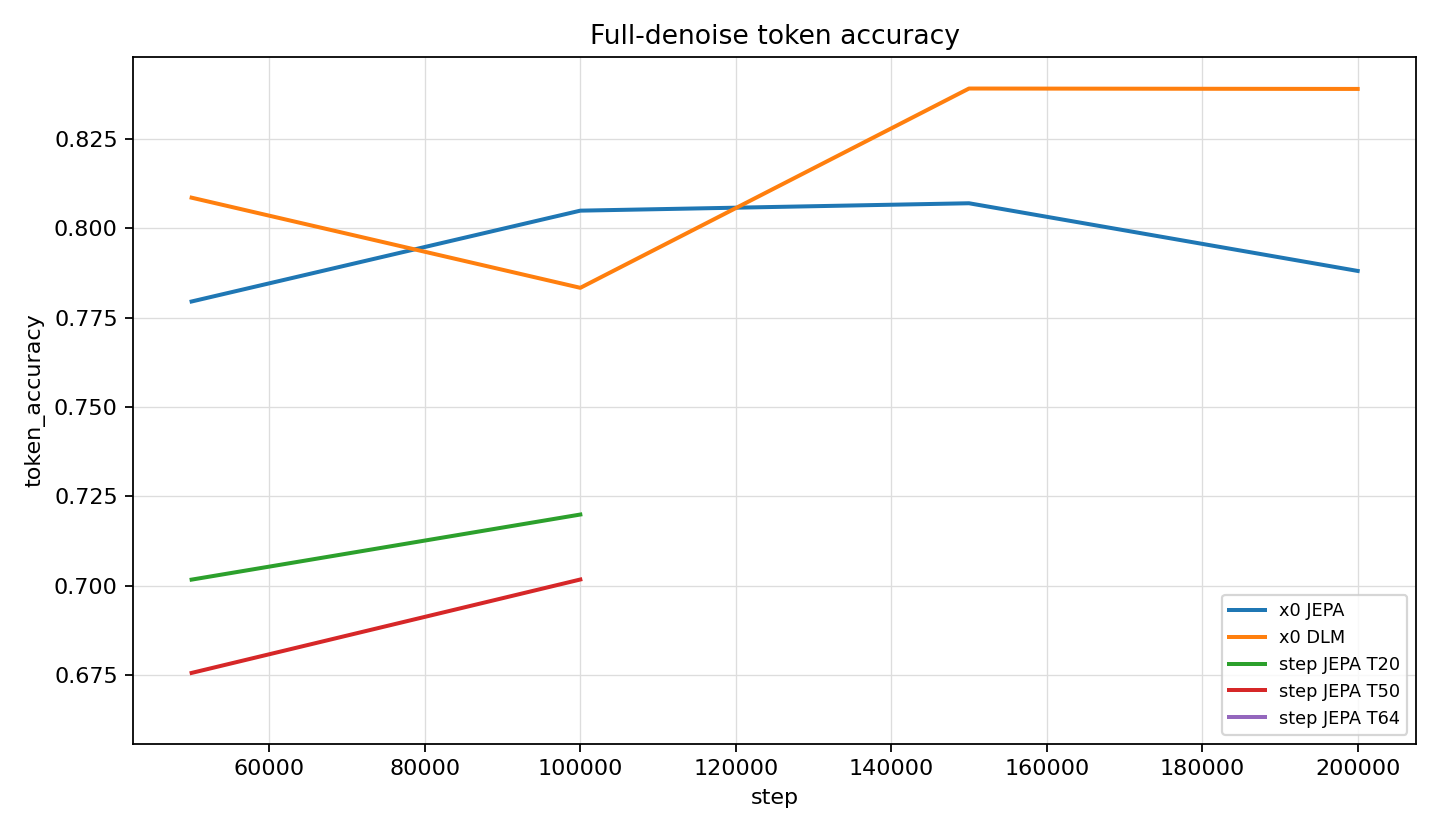
\includegraphics[width=\linewidth]{assets/igsm_full_denoise_token_accuracy.png}
\caption{Periodic full-denoise token accuracy for the major iGSM runs.}
\end{figure}

Additional generated artifacts are stored in
\texttt{docs/assets/igsm\_generation\_samples.md} and
\texttt{docs/assets/posthoc\_summary.md}.  They contain concise sample
generations and compact tables extracted from the posthoc JSON summaries.

\subsection{LANO Replacement}

\begin{table}[h]
\centering
\begin{tabular}{lr}
\toprule
Metric & Value \\
\midrule
Exact reconstruction & 37.3 \\
Token accuracy & 90.2 \\
Grammar validity & 23.5 \\
Edit F1 & 0.214 \\
Edit precision & 0.806 \\
Edit recall & 0.125 \\
\bottomrule
\end{tabular}
\caption{LANO replacement job \texttt{3605204}.  The model is conservative:
high precision, very low recall.}
\end{table}

\subsection{LANO x0 Follow-ups}

The x0 replacement job \texttt{3606651} reached exact 10.7\%, token accuracy
52.6\%, grammar validity 28.0\%, edit F1 0.875, precision 0.859, and recall
0.892.  This flipped the replacement failure mode toward high recall but did not
yet yield good exact or grammar metrics.

Matched-step LANO x0 mask ablations \texttt{3606652\_[0-3]} showed the
denoising LM strongest among those short runs: 25.4\% exact, 63.3\% grammar,
72.9\% token accuracy.  Action-free JEPA was second on exact at 17.1\%, and
action-conditioned JEPA was weaker at 13.1\%.

\section{Qualitative Debug Traces}

\subsection{Original iGSM JEPA Failure Mode}

The JEPA model often generated plausible proof-like text but wrong arithmetic:
\begin{lstlisting}
n=16 start:
<igsm_solution><mask><mask>...

after n=8:
<igsm_solution> Define ... so ... = 13 * ... = 13 * 11 = ...

final:
Define Eel's Haemal Spines as I; so I = 13 * E = 13 * 11 = 15.
<igsm_answer> 11<eos>

expected_answer: 14
predicted_answer: 11
answer_match: False
\end{lstlisting}

\subsection{Original Denoising LM Failure Mode}

The original denoising LM tended to leave masks under full denoise:
\begin{lstlisting}
n=16 start:
<igsm_solution><mask><mask>...

after n=8:
still mostly masks

final:
<igsm_solution><mask><mask>...

predicted_answer: <missing>
answer_match: False
\end{lstlisting}

\subsection{x0 Intermediate Sample at 150k}

During the x0 resume, the model could fill the whole trace but still produced
locally repetitive or arithmetically inconsistent text:
\begin{lstlisting}
gold answer: 18

after n=32:
Define Rotator Cuff's Plasma Cells as <mask>; so <mask> = 17.
Define Colorado Plateau Desert's Zebra as <mask>; so <mask> = <mask> = ...

final:
Define Rotator Cuff's Plasma Cells as j; so j = 17.
Define Colorado Plateau Desert's Zebra as j; so j = j = ...
...
<igsm_answer> 17<eos>

expected_answer: 18
predicted_answer: 17
answer_match: False
\end{lstlisting}
This sample is not the final x0 result and was produced before the submitted
posthoc predictor-decoder/commit-$k$ ablation.  It is useful qualitatively: the
model is no longer simply leaving all masks, but coherence and arithmetic remain
the hard part.

\section{Interpretation}

\paragraph{Schedule was not the first issue.}
The cosine cumulative mask ratio is defensible.  The larger problems were the
objective and sampler: training could reward \texttt{[MASK]}, visible-token CE
dominated, and the sampler could commit \texttt{[MASK]}.

\paragraph{JEPA must be evaluated as JEPA.}
If inference takes tokens straight from the policy head, the latent predictor
loss is only an auxiliary training regularizer.  The corrected inference path
turns JEPA into the intended action-conditioned latent transition model.

\paragraph{x0 JEPA has an action-label limitation.}
When x0 mask JEPA labels every corrupted position \textsc{Replace}, it does not
teach a policy to choose which masked tokens to reveal first.  The sampler can
still choose by confidence, but the action labels are not a stepwise decision
process.  This is why the stepwise JEPA ablation was added.

\paragraph{Stepwise JEPA is not the same as SOTA masked diffusion.}
For the denoising LM, the SOTA-like baseline is x0 masked-token prediction.  For
JEPA, stepwise training is a targeted ablation: it asks whether an
action-conditioned latent model benefits from explicit next-state supervision
and KEEP/REPLACE action choices.

\paragraph{Insert/delete needs a richer action space.}
The current fixed-length action tensor can represent parallel replacement, but
true variable-length edits require gap actions.  The proposed clean extension is
\textsc{InsertAfter}, plus \textsc{Delete}, \textsc{Replace}, and \textsc{Keep}.
The forward noising process should be an MDP over token sequences whose reverse
actions are invertible: random replacement reverses to \textsc{Replace}, random
deletion reverses to \textsc{InsertAfter} at the previous retained token, and
random insertion reverses to \textsc{Delete}.  This has not been implemented in
the submitted jobs because it needs gap-indexed supervision and sequence-length
handling.

\section{Next Experiments}

\begin{enumerate}[leftmargin=*]
\item Finish \texttt{3612683\_2}/\texttt{3612683\_3} and the dependent
  \texttt{3612684}/\texttt{3612685} chains so final T64 and all-checkpoint
  stepwise curves are available.
\item Analyze \texttt{3615623}: top-M/top-K proposal coverage, factorized
  position-vs-token oracle modes, and DLM-token proposer modes.
\item Analyze \texttt{3615624}: larger oracle-MPC candidate sets, horizons, and
  latent-only vs materialized re-encode planning.
\item Analyze \texttt{3615625}: whether a learned value head can approximate
  oracle-goal latent energy well enough to replace oracle scoring.
\item Analyze \texttt{3615643}: whether rollout latent loss repairs stepwise
  inference collapse.
\item If proposal coverage is poor, train a stronger token proposer or distill
  the x0 denoising LM token head into the stepwise policy.
\item If proposal coverage is good but generation remains poor, prioritize
  on-policy repair/scheduled sampling and value-based action selection.
\item Design and implement the variable-length edit MDP with
  \textsc{InsertAfter}, \textsc{Delete}, \textsc{Replace}, and \textsc{Keep}.
\end{enumerate}

\section{References}

\begin{itemize}[leftmargin=*]
\item D3PM: Structured Denoising Diffusion Models in Discrete State-Spaces,
  \url{https://arxiv.org/abs/2107.03006}.
\item SEDD: Discrete Diffusion Modeling by Estimating the Ratios of the Data
  Distribution, \url{https://arxiv.org/abs/2310.16834}.
\item MD4: Simplified and Generalized Masked Diffusion for Discrete Data,
  \url{https://arxiv.org/abs/2406.04329}.
\item MDLM: Simple and Effective Masked Diffusion Language Models,
  \url{https://arxiv.org/abs/2406.07524}.
\item SMDM: Scaling up Masked Diffusion Models on Text,
  \url{https://arxiv.org/abs/2410.18514}.
\item LLaDA: Large Language Diffusion Models,
  \url{https://arxiv.org/abs/2502.09992}.
\item MaskGIT: Masked Generative Image Transformer,
  \url{https://arxiv.org/abs/2202.04200}.
\end{itemize}

\end{document}
